\section{Progress}

\subsection{Programmer View Implementation}
\subsubsection{Implementation From the Benchmark}

The Parboil benchmark provides datasets to run the programmer view
implementation. In their github repository~\cite{Rub1}, we can find
documentation of this benchmark. After cloning the whole Parboil to local, under
the Parboil folder, I ran the benchmark by the following command:
$$\text{./parboil run mri-q cpu small}$$ Here, ``small“ means the dataset is
stored under ``small" folder, whose input image size is 32*32*32. I have also
ran the test for ``large", whose input image size is 64*64*64. The image size of
the largest dataset is 128*128*128.  The bigger the input data size, the higher
precision of the reconstructed image.The running time for small and large are
around 4.7s and 18.7s, respectively. But for the ``128x128x128" input dataset,
the run time is 186685s$ \sim$ 2.2 days. This implementation was done on the
socp03.cs.columbia.edu google cloud server with two cores.

\begin{table}[]
    \centering
    \begin{tabular}{c|c|c|c}
    \hline
    \hline
       name  & image size & \# of pixels & K-space dimension  \\
        \hline
    \hline
        small  & 32*32*32 & 32768 & 3072 \\
        large & 64*64*64 & 262144 & 2048\\
        128*128*128 & 128*128*128 & 2097152 & 2097152\\
        \hline
        \hline
    \end{tabular}
    \caption{Datasets of MRIQ from Parboil Benchmark}
    \label{tab-1}
\end{table}
\subsubsection{Implementation From Modified C Code}

In order to have a comparison between hardware implementation and software
implementation, we need to run the software version on the processor of our SoC
on FPGA. So I modified the software C code and put this implementation as a
function call in the sw/linux/app/mriq.c code.\\

\subsection{Design MRIQ Accelerator in SystemC}

The MRIQ application is to compute the Q matrix. Each element of the Q matrix is
a complex number with imaginary and real part. The input data can be divided
into two groups. One group is coordinates information from frequency space,
which is called k-space data. The other group is the sampling positions in 3-D
space, which is sometimes called sampling space data. There are 5 variables from
k-space, and 3 variables from the sampling space. Each pair of output is
computed by using one sampling space point accumulating through the whole
k-space. For the ``small" and ``medium" dataset in Table \ref{tab-1}, it has 15
K words at most for k-space data. The storage requirement is 60 K Bytes if data
width is 32-bit. The whole k-space data can be stored into PLM. While for the
``large" dataset, it is 20 M words, which is 80 M Bytes. For some potential
unknown applications with even higher image resolution, the storage requirement
for k-space data could be larger. The storage cost may be so high that we want
to sacrifice speed. For a specific application, the designer should balance the
storage cost and speed requirements. For the MRI-Q matrix application, the Q
matrix computation is not in real-time, so we may want to save the cost of
storage and compromise on speed. Thus we need at least two architectures to deal
with different input image sizes. One is called A0 dealing with small k-space
data, the other is A1 dealing with large k-space data.\\



\subsubsection{Configuration Parameters}

There are two parameters provided by the benchmark, numX and numK. Since we
might deal with one batch data one time, we set four parameters in total:
batch\_size\_x, batch\_size\_k, num\_batch\_x, and num\_batch\_k. And they have
the following relationships with numX and numK:

    $$numX = batch\_size\_x * num\_batch\_x$$
    $$numK = batch\_size\_k * num\_batch\_k$$

$batch\_size\_x$ denotes the size of one batch for sampling space
data. $num\_batch\_x$ indicates how many batches needed to load the whole
sampling space data. These four configuration parameters are suitable for both
A0 and A1 architecture. While for A0 architecture, $num\_batch\_k$ is always 1,
and $batch\_size\_k$ should be equal to $numK$.\\

\subsubsection{PLM Design}

The private local memories of accelerator is generated by "memgen" script
provided by ESP. We need a script to tell memgen what kind of PLMs we
need. There are three aspects we need to consider when designing PLM for MRI-Q
accelerator. Firstly, the word size of the PLM. Input variables from sampling
space and output have the same size, while PLMs storing k-space data should have
a different word size. Additionally, PLMs storing k-space variables customized
for A0 architecture should have size of $numK$, while it should be
$batch\_size\_k$ for A1. Secondly, DMA width of the processor core. In order to
maximize the latency performance, we can customize ports of PLMs to work with
different processor cores. For example, Ariane core has 64-bit DMA width, the
PLM should provide two writing ports when loading data into PLM in
parallel. while one port is enough for Leon3 core with 32-bit DMA
width. Thirdly, parallelism level. In compute phase, how many data we can access
in parallel is determined by number of the corresponding PLM ports. For example,
if we wanted to do 4 computation in parallel, the PLM which stores the input
data should have 4 reading ports. Then we should specify in the
hw/mriq\_directives.hpp file that what memory we want to use under what
conditions.


\subsubsection{Data Type}

Since the FPGA can not process floating-point data directly, we need to do
various data conversions in both the accelerator and the testbench. fpdata.hpp
file defines functions used to do datatype conversions, including int2fp(),
fp2int(), fp2bv(), bv2fp(). The data conversion flow is concluded in
Fig.\ref{fig-data-convert}. In the testbench, data in floating-point type read
from files is converted to fixed-point representation, then converted to sc\_bv
to be transported through the network-on-chip. In accelerator, data in sc\_bv
type is converted to sc\_int to be stored in PLM. In computation phase, sc\_int
data is converted back to fixed-point representation. After computation
finished, The fixed-point data needs to be converted back to sc\_int to be
stored in PLM. Then, it is further converted to sc\_bv to be transported back to
the testbench for validation. In testbench, sc\_bv is converted to fixed-point
representation. and further converted to floating-point type to be compared with
the golden output data. \\

\begin{figure}[t]
\centering
\captionsetup{justification=centering, format=hang}
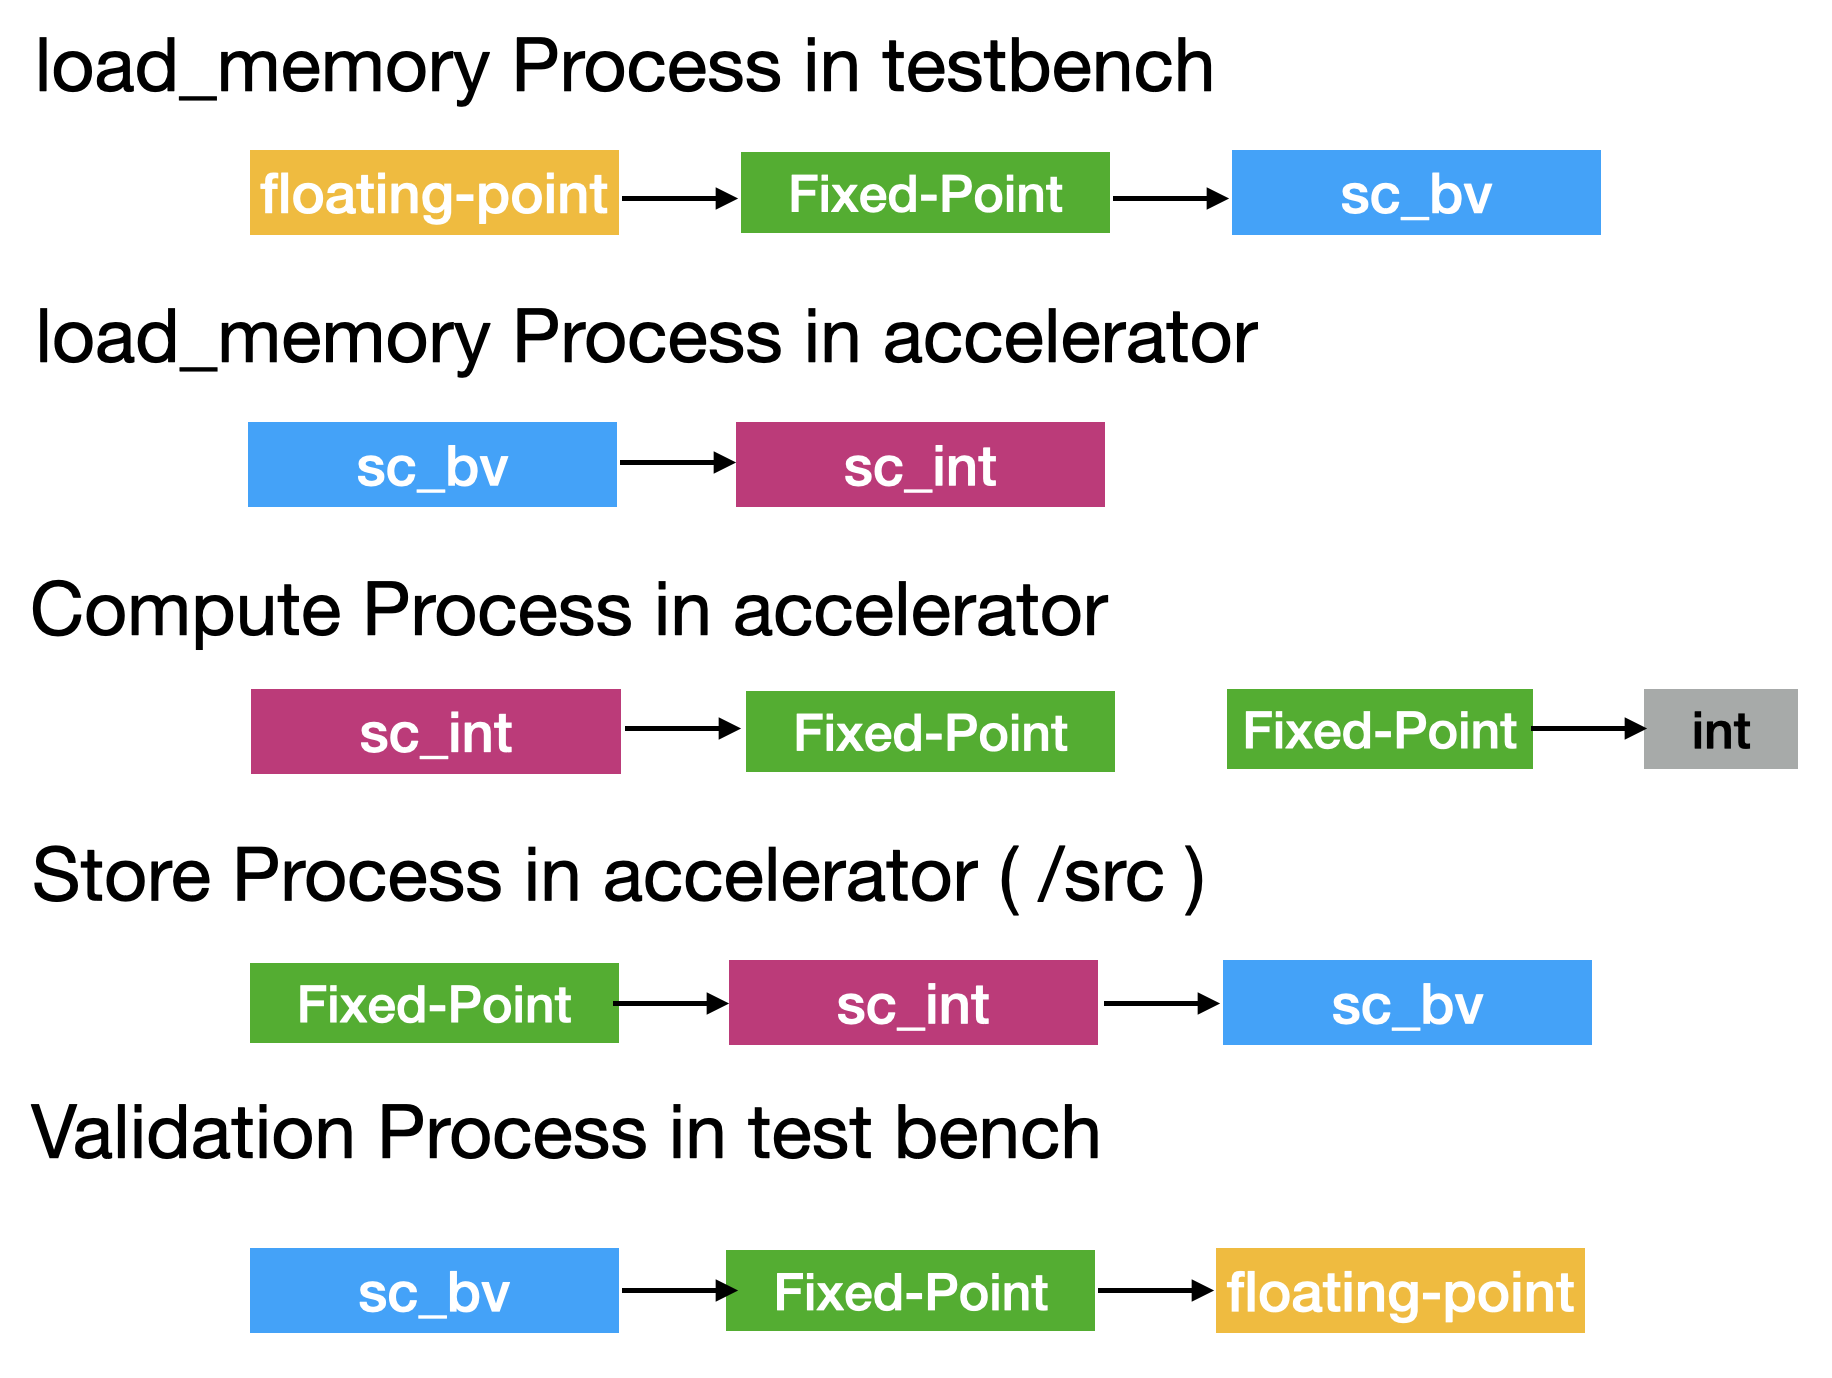
\includegraphics[width=\columnwidth]{figures/data-conversion}
\caption{Data conversion in testbench and accelerator}
\label{fig-data-convert}
\end{figure}



\subsubsection{Functions}

There are four functions essential to MRI-Q accelerator design. In load process,
\textit{load\_data()} function is to load data into different PLMs. This
function loads "len" number of words, starting with dma address "dma\_addr",
into a PLM with name "array". In this function, dma\_info is configured first,
including dma\_addr, dma\_length, and dma\_size. Then it stores data from
dma\_read\_chnl to PLM "array".
%
$$\mathrm{load\_data(array[], dma\_addr, len)}$$
%
The second function is \textit{store\_data}, which is the counterpart of
load\_data(). It sends data stored in "array" PLM through dma\_write\_chnl to
the testbench.
%
$$\mathrm{store\_data(array[], dma\_addr, len)}$$
%
The third function is \textit{computeQ} which is to compute a pair of output
data with the whole k-space variables and one sampling space data point (x, y,
z). In computeQ, there are three tasks being pipelined. The first task is
reading data from PLM into registers kx, ky, kz, phiR, and phiI. The second task
is to do the computation part. The third taks is to accumulate the intermediate
results. After the loop finishes, it stores the accumulated results into two
memory addresses pointed by pointers Qr and Qi.
%
$$\mathrm{computeQ(x, y, z, batch\_size\_k, pingpong\_x, sin\_table, *Qr, *Qi)}$$

\begin{figure}[t]
\centering
\captionsetup{justification=centering, format=hang}
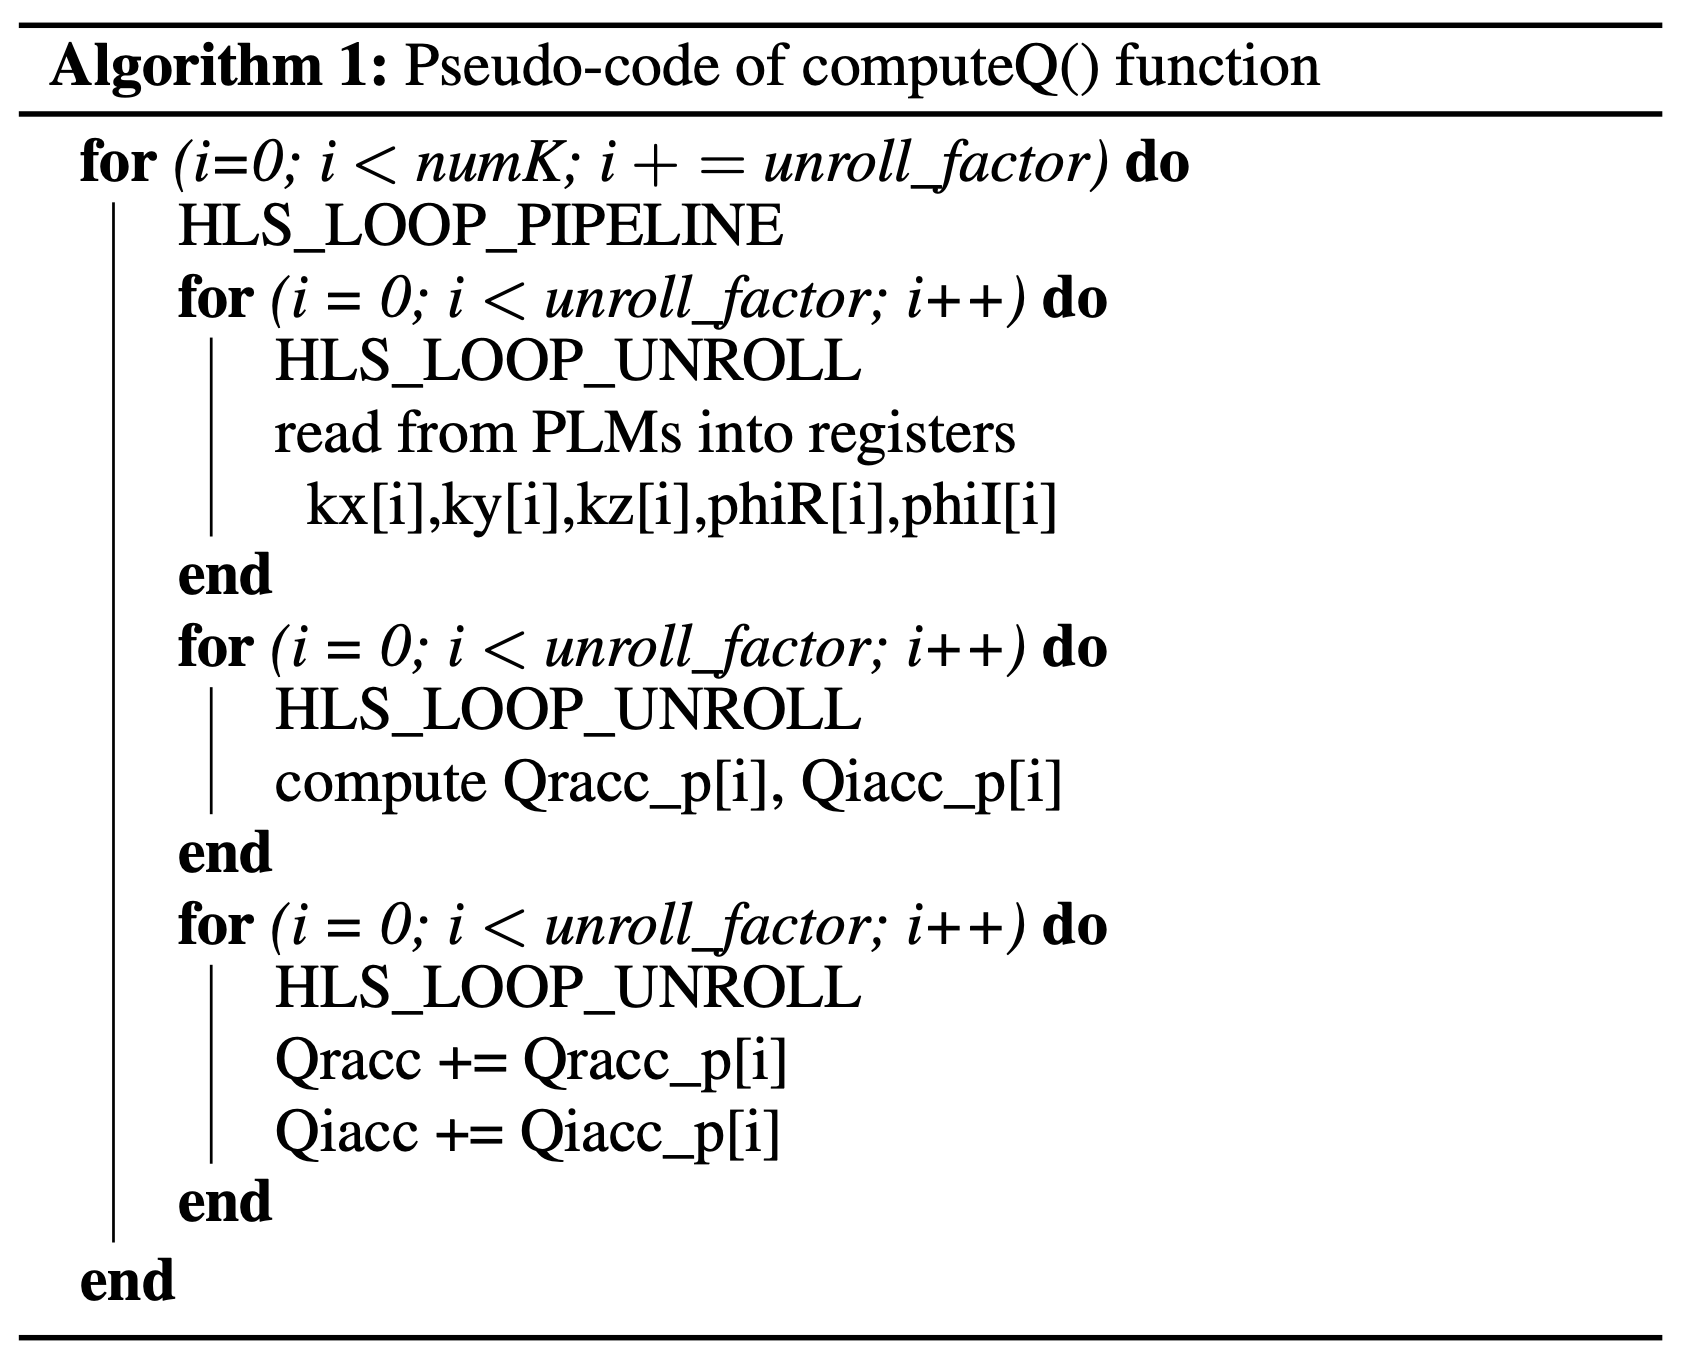
\includegraphics[width=\columnwidth]{figures/computeQAlgorithm}
\label{fig-data-convert}
\end{figure}

The fourth function is \textit{mySine} which is to compute the sine value of an
input.
%
$$\mathrm{mySinf(angle, sin\_table)}$$
%
The algorithm in Fig.\ref{fig-1} shows
that it needs to compute triangular functions, sine and cosine. Since Stratus
HLS doesn't provide sine and cosine function, we implemented a sine function
\textit{mySine}. We firstly convert any input value to $0~\pi/2$ range, $x$,
then find the closest data point to $x$ in the sin\_table, then do interpolation
to get sin(x).  \\

\subsubsection{Processes}

In the main hardware design source file mriq.cpp, we have three processes,
load\_input, compute\_kernel, and store\_output. load\_input handshakes with
compute\_kernel. compute\_kernel handshakes with store\_output. These three
processes are pipelined in the background. For both A0 and A1 architectures, we
are utilizing ping-pong buffers to store sampling space variables (x, y, z) and
(Qr, Qi). A flag pingpong\_x is to tell each processes whether we should read
from or write to plm\_var\_ping or plm\_var\_pong memory. For A1 architecture,
we also need ping-pong buffers to store k-space variables. Thus we need another
flag pingpong\_k as a local variable in each process. Conditional loading in the
load\_input process is implemented. We have a counter variable counting how many
times load\_input process has been implemented. Whenever we load one batch of
sampling space variables, we need to load k-space variables for $num\_batch\_k *
batch\_size\_x$ times, and we flip pingpong\_k flag and handshake with
compute\_kernel process for every loading. Then we flip pingpong\_x and reset
the counter in load\_input process. After the computation of the current batch
of sampling space variables finishes, we flip pingpong\_x flag once and
handshake with store\_output process in compute\_kernel process. \\

\subsection{Testbench Design}

The ESP provides skeleton code for the testbench design. We only need to fill in
customized code in each function. In tb/system.hpp file, it defines a class
system\_t. In this class declaration, there is a constructor function, and other
members. For example, configuration parameters to the accelerator, variables
used by different methods, and methods. Here we declare an additional method
used by load\_memory function, which is load\_mem() method. In system.cpp file,
we have four methods definitions. In load\_memory(), we initialize the necessary
parameters first, then fill the "mem" variable with input data and fill the
"gold" pointer with golden output data. Since the accelerator can only deal with
fixed-point data, we convert floating-poing data to sc\_bv to be transported to
the accelerator. In dump\_memory(), we convert and store the output sent from
the accelerator to a pointer variable "out" with floating-point type. In
validate(), we compare "out" with "gold" to verify the accelerator
design. \\ \\ We define some helper functions in a separate folder, "common"
folder. In the testbench design, we used init\_parameter() and
validate\_buffer(), defined in utils.h file. These two helper functions are also
used in software testing application code.\\

\subsection{Software Testing Applications}

ESP enables two testing on FGPA. One is bare metal application testing and the
other is testing the accelerator with Linux OS. These two applications are in
sw/ folder. \\ \\ For the bare metal application, we need to fill in code in
init\_parameters(), init\_buf() and validate\_buf(). Since bare metal
implementation doesn't support many C librabries, we can't use init\_buffer
function in common/utils.h file. We generated testing input data beforehand and
included it as a file. While in validate\_buf function, we first convert output
sent from the accelerator from fixed-point data to floating-point data by using
fixed32\_to\_float() function provided by fixed\_point.h. Then use
validate\_buffer() function from common/utils.h to validate the
output. \\ \\ For linux application, we also only need to fill customized code
in init\_parameters(), init\_buf(), and validate\_buf() function, same as the
bare-metal application except the init\_buf() function. Since we run the test
program on linux OS, the init\_buf can use the function init\_buffer() in
common/utils.h, which reads input data from file. We can also test the execution
time of software program running on the processor tile of SoC which is
prototyped on the FPGA. When running the linux application, we pass three
arguments: name of input File, name of output file, and the answer to whether we
want to run software program with "0" indicating "no" and "1" indicating "yes".
\\
\subsection{Testing Results}

The testbench can help us debugging our accelerator at design phase. When we
don't have "\#if" directives, we can run behavioral simulation by running make
target "make mriq\_stratus-exe". This will check if our accelerator has the
expected behavior. Then we can generate RTL with "make mriq\_stratus-hls" and
simulate RTL with the testbench. When we use "\#if" directive to generate
multiple RTL implementations, the above three make targets won't work
correclty. Then we need to use the debugging method provided on the ESP
tutorial, which is to simulate one specific RTL with "make debug\_<RTL
name>". For example, if we want to test A1 architecture with DMA width as 64 and
parallelism level as 4, we can run "make debug\_BASIC\_P4\_A1\_DMA64\_V". The
running result is shown in Fig.\ref{fig-3}.  \\

\begin{figure}[ht]
\centering
\captionsetup{justification=centering, format=hang}
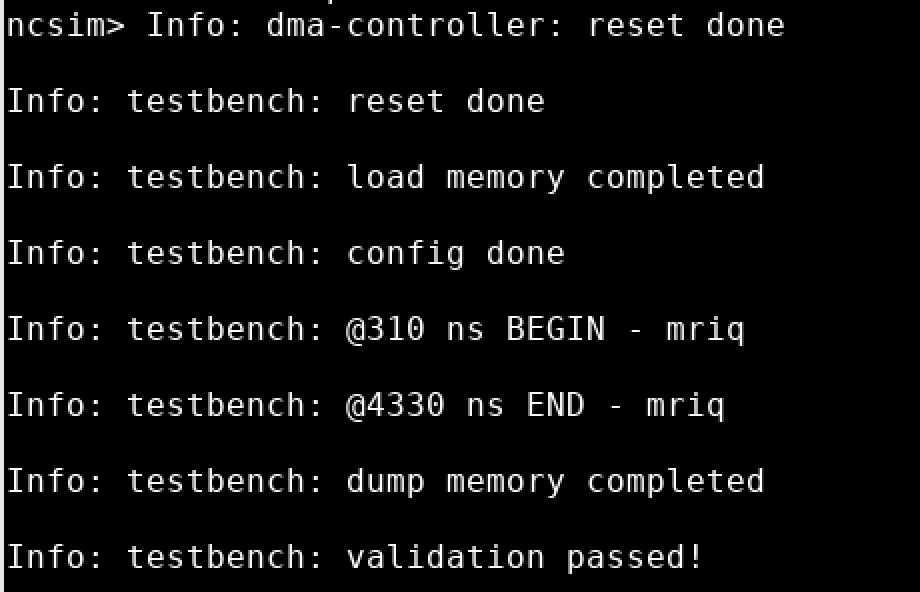
\includegraphics[width=0.75\columnwidth]{figures/debug-sim-A1-4-4-2-2}
\caption{RTL simulation (BASIC\_P4\_A1\_DMA64\_V)}
\label{fig-3}
\end{figure}

After we finish the software testing program design, we can also simulate and
test the bare metal application, and run the Linux application after booting the
FPGA with Linux image. For the baremetal application, for example, we test
"P4\_A0\_DMA64" RTL on FPGA, the result is shown in Fig.\ref{fig-barec-app}. If
we generated Linux image and registered the mriq\_stratus accelerator as a
device driver, we can test the linux app on FGPA. The running result is shown in
Fig.\ref{fig-linux-app}. Fig.\ref{fig-linux-app}-(a) shows that we also ran the
software program on the SoC core, and the execution time is roughly 10 times
slower than the hardware accelerator on a small testing data.

\begin{figure}[t]
\centering
\captionsetup{justification=centering, format=hang}
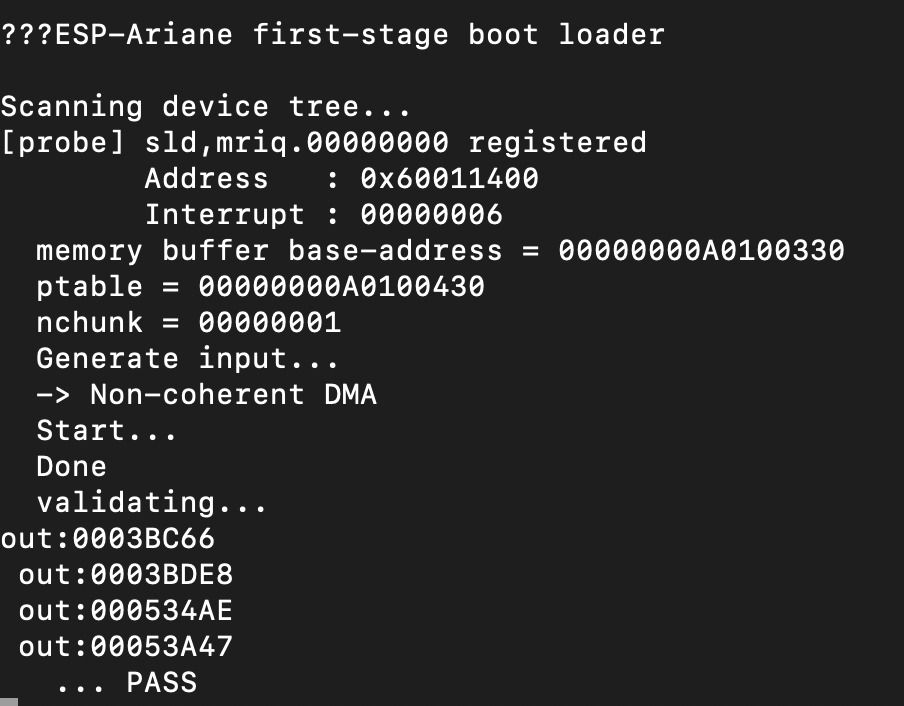
\includegraphics[width=\columnwidth]{figures/barec-fpga}
\caption{Running bare metal app on FPGA}
\label{fig-barec-app}
\end{figure}

\begin{figure}[t]
\centering
\begin{subfigure}{.5\columnwidth}
\centering
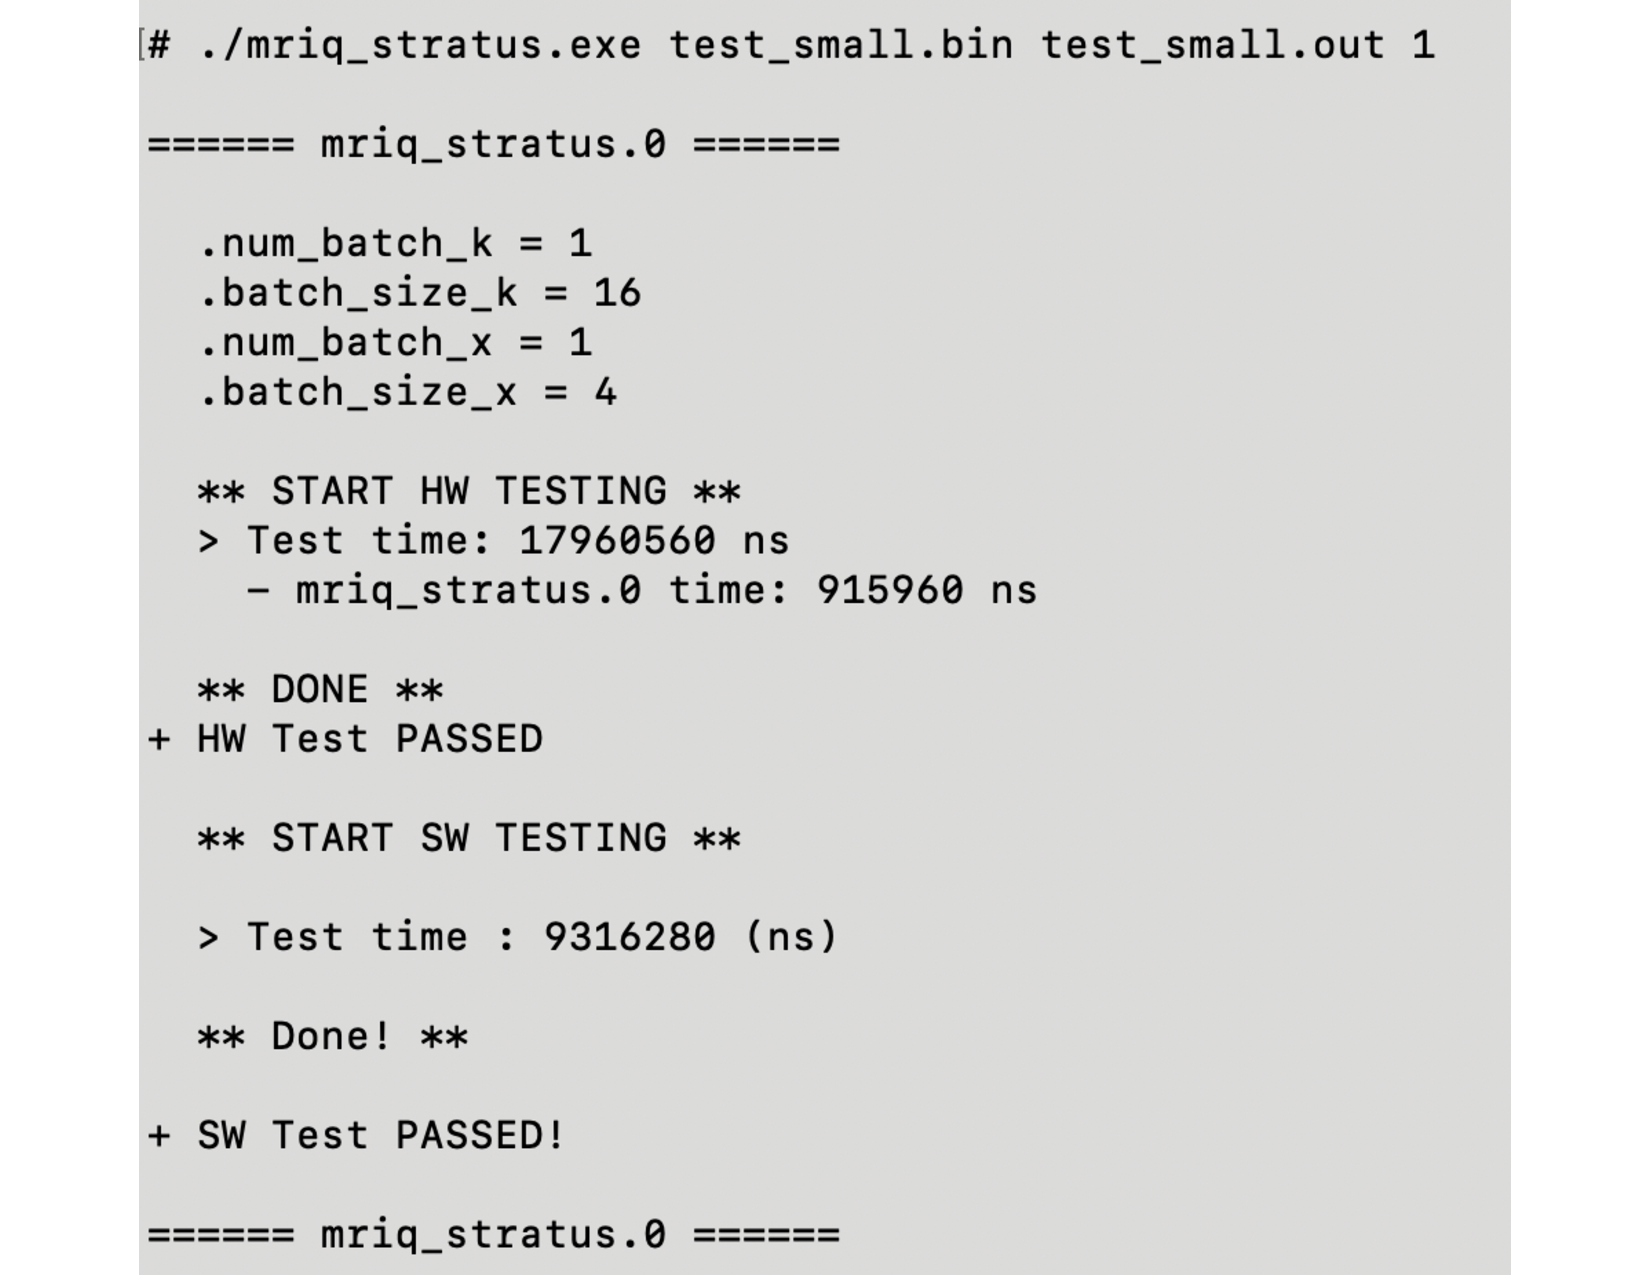
\includegraphics[width=\columnwidth]{figures/linux-run-sw}
\caption{w/ running sw}
\end{subfigure}%
\begin{subfigure}{.5\columnwidth}
\centering
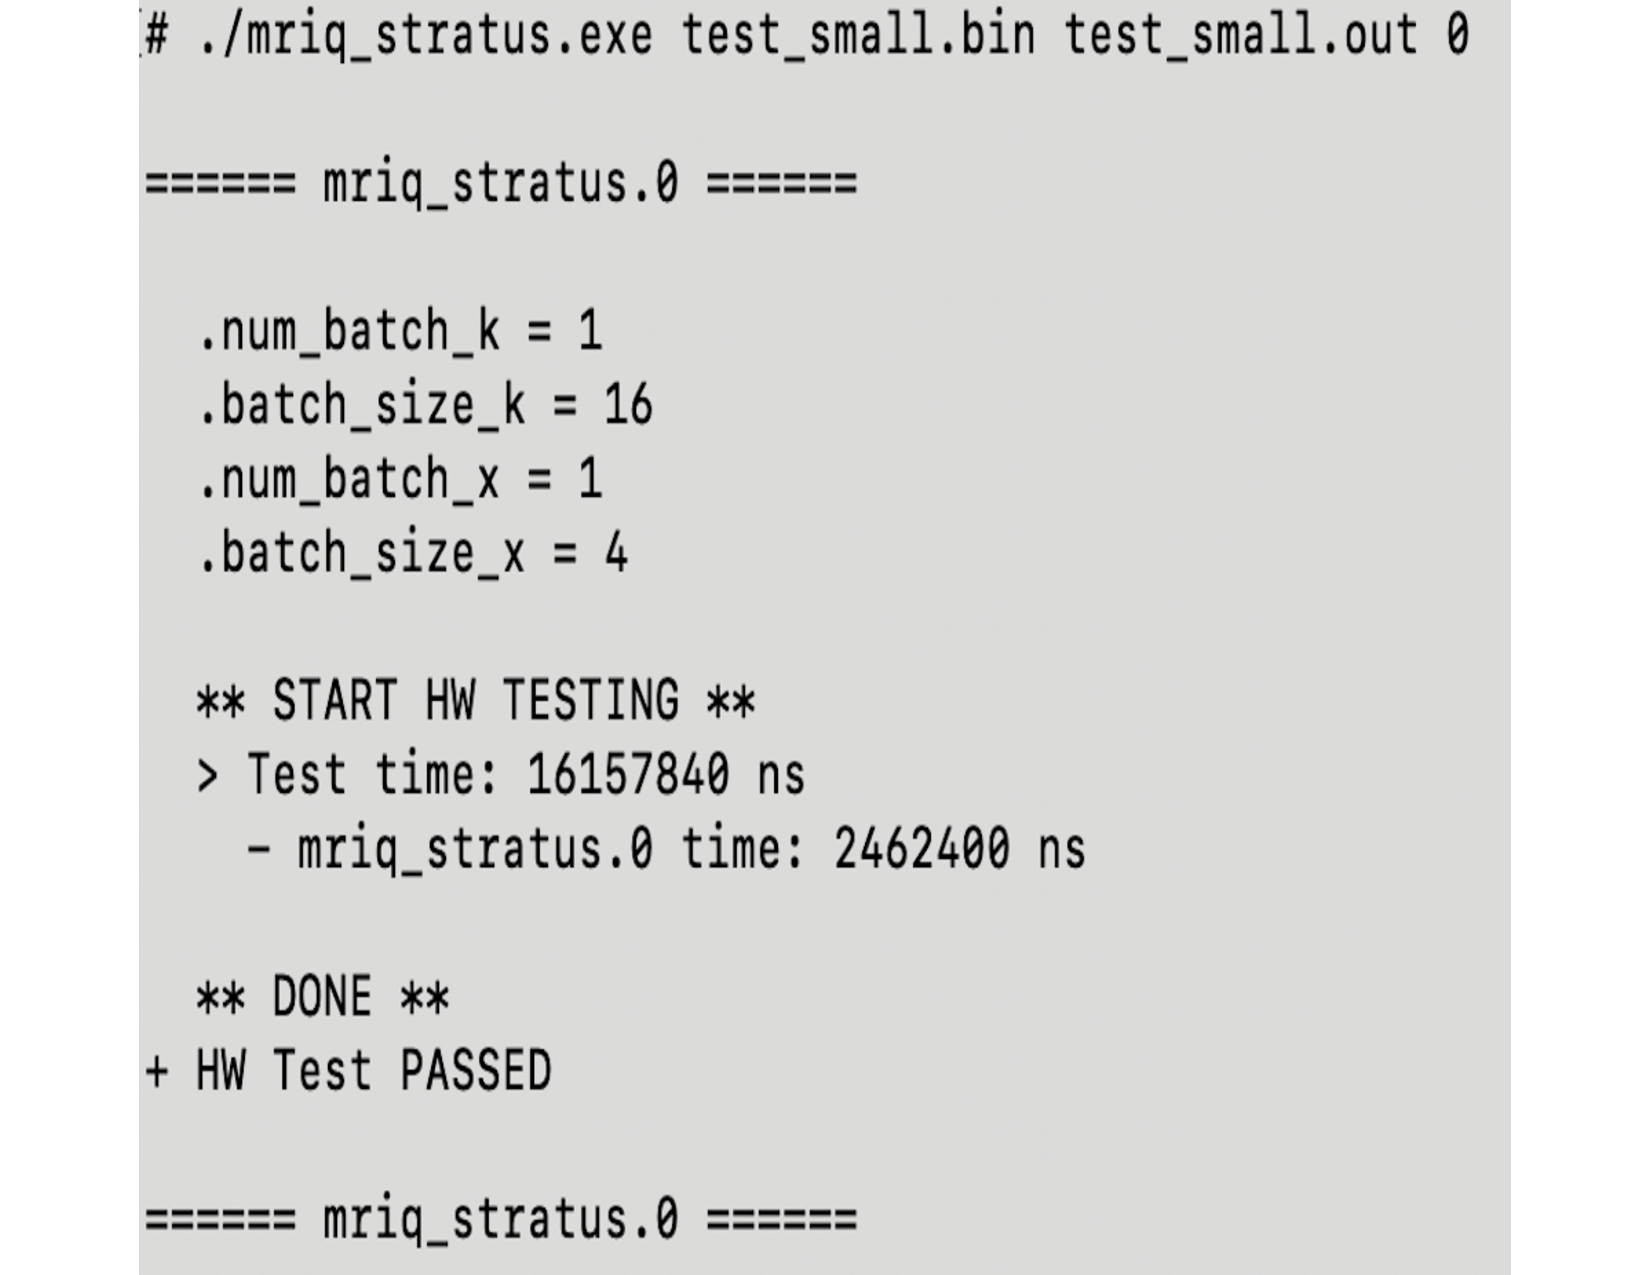
\includegraphics[width=\columnwidth]{figures/linux-app-wo-run-sw}
\caption{w/o running sw}
\end{subfigure}
\caption{Running Linux app on FPGA}
\label{fig-linux-app}
\end{figure}
